\documentclass[titlepage=true, parskip=full]{scrartcl}
\usepackage[utf8]{inputenc} % use utf8 file encoding for TeX sources
\usepackage[T1]{fontenc}    % avoid garbled Unicode text in pdf
\usepackage{palatino}	      % because "Computer Modern" standard font is illegible
\usepackage{mathpazo}
\usepackage[ngerman]{babel}  % german hyphenation, quotes, etc
\usepackage{hyperref}       % detailed hyperlink/pdf configuration
\hypersetup{                % ‘texdoc hyperref‘ for options
	pdftitle={PSE: Pflichtenheft},%
	bookmarks=true,%
}
\usepackage{graphicx}       % provides commands for including figures
\usepackage{csquotes}       % provides \enquote{} macro for "quotes"
\usepackage[nonumberlist, numberedsection]{glossaries}     % provides glossary commands
\usepackage{enumitem}
\usepackage{tikz}
\usepackage{tikz-uml}
\usepackage{comment}
\usepackage{array}
\usepackage{longtable}
\usepackage{hhline}
\usepackage{needspace}

% fix hyphenation
\hyphenation{Log-out Log-in Ak-tions Ak-tion ge-öff-net}



\makeglossaries

\title{Studienplanung als Generierung von Workflows mit Compliance-Anforderungen: Planerstellung und Visualisierung}
\subtitle{Pflichtenheft}
\author{Daniel Jungkind \and Ulrike Rheinheimer \and Hannes Kuchelmeister \and Samuel Teuber \and Nada Chatti \and Tim Niklas Uhl}
\date{30. November 2016}

\begin{document}

\maketitle
\tableofcontents
\pagebreak

%
% % Hier beginnt die Gliederung des Pflichtenhefts
\section{Einleitung}
Der Implementierungsbericht des Projekts „Studienplanung als Generierung von Workflows mit Compliance-Anforderungen: Planerstellung und Visualisierung“ beschreibt die Umsetzung des zuvor im Pflichtenheft und Entwurf spezifizierten Projekts. In über ????? Zeilen Java-, Javascript-, HTML- und CSS-Code liegt jetzt eine fertige, nur noch zu optimierende Anwendung vor. In diesem Bericht möchten wir dabei auf implementierte und ausgelassen Features eingehen, Änderungen beschreiben und begründen, und die Implementierungsphase (einschließlich aller durchgemachten Nächte) reflektieren.
Zusammenfassend ist dieser Bericht Ende einer arbeitsintensiven, aber erfolreichen Phase, die als Endprojekt ein einmalig sinnvolles, dringendnotweniges und jedem Studenten zu empfehlendes Studienplanungshilfsmittel zur Verfügung stellt.



 
\section{Zielbestimmung}

\subsection{Musskriterien}
\begin{itemize}[nosep]
	\item Webbasierte Benutzeroberfläche:
	\begin{itemize}[nosep]
		\item Benutzerorientiert 
		\item Nutzer: Studenten
	\end{itemize}
	\item Funktionen:
	\begin{itemize}[nosep]
		\item Login
			\begin{itemize}[nosep]
					\item Speichern von: Studiengang, Studienbeginn, bestandene und begonnene Prüfungsleistungen, bereits erstellte Studienpläne
				\end{itemize}
		\item Generierung $\rightarrow$ Erstellung/Vervollständigung von möglichen Studienplänen
		\item Berücksichtigung von Constraints:
		\begin{itemize}[nosep]
			\item Unterscheidung zwischen Pflicht- und Wahlveranstaltungen
			\item Wahl eines Vertiefungsfaches
			\item Abhängigkeiten zwischen Modulen (Voraussetzungen, Zusammenhänge, Überschneidungen)
			\item zur Verfügung stehende Semesteranzahl
			\item gewünschte Module
			\item bisheriger Studienverlauf
		\end{itemize}
		\item Studienpläne manuell bearbeiten ( Module einfügen / löschen)
		\item Speichern und Löschen von Studienplänen
		\item Verifizierung von Studienplänen
		\begin{itemize}[nosep]
			\item Ermöglicht dieser Studienplan ein erfolgreiches Abschließen des Studiums?
			\item Sind alle Constraints erfüllt?
		\end{itemize}
	\end{itemize}
	\item Gegebene Algorithmen zur Generierung und Verifizierung einbinden
	\item Modularität
	\item Modular erweiterbar
	\item Objektorientierung
	\item Studienplan als Workflow modellieren
	\begin{itemize}[nosep]
		\item Module/Lehrveranstaltungen als Aktivitäten
	\end{itemize}
	\item Module modellieren mit folgenden Details: Name, ECTS-Punkte, Angebot im Sommer- oder Wintersemester, Art der Veranstaltung
	\item Module auf einen Studienplan bezogen positiv oder negativ bewerten und dies dem Studienplan zugeordnet speichern
	\item Modulübersicht
		\item Alle Module in einer Liste
			\begin{itemize}[nosep]
				\item betrachten können
				\item Suche nach Namen
				\item In Studienplan ziehen können
			\end{itemize}
\end{itemize}

\subsection{Wunschkriterien}
\label{subsec:project_goals-wunschkriterien}
\begin{itemize}[nosep]
	\item  Login über Shibboleth	
	\item Benennung von Studienplänen
	\item Duplizieren von Studienplänen
	\item Studienpläne exportieren
	\item Vergleichsansicht für 2 (mehrere?) Pläne 
	\item Modulübersicht
	\begin{itemize}[nosep]	
		\item Suche durch folgende Filter spezifizierbar : 
		\begin{itemize}[nosep]
			\item Angebotenes Semester
			\item Veranstaltungsart
			\item Fachrichtung
			\item Pflicht-/Wahlmodul
			\item Kategorie
			\item ECTS-Bereich
		\end{itemize}
		\item Detailansicht eines Moduls für Details
	\end{itemize}
	\item Rückgängig-Button
	\item Weitere Constraints
	\begin{itemize}[nosep]
		\item benötigte ECTS-Punkte
		\item ausgeschlossene Module
	\end{itemize}
	\item Studienpläne mit anderen teilen
\end{itemize}
\subsection{Abgrenzungskriterien}
\begin{itemize}[nosep]
	\item kein Notenportal
	\item keine Vernetzung zwischen Studenten
	\item keine Schnittstelle zum Prüfungsportal
	\item keine Unterstützung von parallelen Studiengängen
	\item der Nutzer kann keine eigenen Module erstellen
	\item Vorlesungsuhrzeiten und -details sind unerheblich
	\item nicht handyfähig (bei Bedarf: per App)
	\item Lösungsalgorithmen werden nicht entworfen
	\item Sonderanträge können nicht berücksichtigt/eingebracht werden
	\item was nicht im Modulhandbuch genannt ist, ist nicht möglich
\end{itemize}

\section{Produkteinsatz}

\subsection{Anwendungsbereiche}

\subsection{Zielgruppen}

\subsection{Betriebsbedingungen}

\section{Produktumgebung}
\begin{itemize}
	\item Eine Client-Server-Architektur
	\item Der Client ist webbasiert
\end{itemize}
\subsection{Software}
\begin{itemize}
	\item Serverseite
	\begin{itemize}
		\item mySQL-Installation
		\item Apache-Tomcat-Webserver
	\end{itemize}
	\item Clientseite
	\begin{itemize}
		\item Betriebssystem mit grafischer Benutzeroberfläche
		\item \gls{Internetbrowser}, Referenzstandard Mozilla Firefox 48
	\end{itemize}
\end{itemize}
\subsection{Hardware}
\begin{itemize}
	\item Serverseite
	\begin{itemize}
		\item Leistungsstarker Standardrechner
	\end{itemize}
	\item Clientseite
	\begin{itemize}
		\item Endgerät mit einer Bildschirmbreite von mindestens 1200 Pixeln und einer Bildschirmhöhe von mindestens 800 Pixeln (z.B. PC, Tablet)
	\end{itemize}
\end{itemize}
\subsection{Orgware}
\begin{itemize}
	\item Das Endgerät benötigt eine funktionierende Netzwerkverbindung zum WorldWideWeb
\end{itemize}

\section{Funktionale Anforderungen}

	\subsection{Grundfunktionen}
	\begin{itemize}[nosep]	
		\item [FA10] Anzeigen eines Login-Fensters
		\item[FA20] Login mit den KIT-Daten über den Shibboleth Identity Pro-vider
		\item [FA30]Eingabe (in einem Registrierungs-\gls{Wizard}) und Speicherung von
		\begin{itemize}[nosep]
			\item Studiengang
			\item Studienbeginn
			\item bestandene Prüfungsleistungen
			\item begonnene Prüfungsleistungen
		\end{itemize}
		\item [FA40] Erstellen von Studienplänen
		\item [FA41]Anzeigen einer Übersicht aller gespeicherten Studienpläne
		\item [FA50] Generierung von Studienplänen unter Berücksichtigung
			\begin{itemize}[nosep]
			\item von Pflichtveranstaltungen
			\item der Wahl eines Vertiefungsfaches
			\item von Abhängigkeiten zwischen Modulen
			\item der zur Verfügung stehenden Semesteranzahl
			\item gewünschter \glspl{Modul}
			\item des bisherigen Studienverlaufs
			\end{itemize}
		\item [FA60] Verifizierung von Studienplänen
		\item [FA70] Studienpläne manuell bearbeiten
		\item [FA71] 
		\item [FA80]Speichern und Löschen von Studienplänen
		\item[FA90] Bearbeitungsansicht mit einem Studienplan und Modulübersicht anzeigen 
		\item[FA110] \glspl{Modul} suchen (Volltextsuche)
		\item[FA120] \glspl{Modul} einem Studienplan zufügen
		\item[FA125] \glspl{Modul} studienplanbezogen positiv oder negativ bewerten (berücksichtigt Generierung)
		\end{itemize}
	\subsection{Erweiterte Funktionen}
		\begin{itemize}[nosep]
		\item [FA130] \glspl{Modul} filtern
		\item[FA135] einzelne Module anzeigen (Detailansicht)
		\item [FA140]	Benennung von Studienplänen
		\item [FA150] Duplizieren von Studienplänen
		\item [FA160] Studienpläne exportieren
		\item [FA170] Studienpläne mit anderen teilen
		\item[FA180] Studienpläne vergleichen
		\item [FA190] "Rückgängig machen" der jeweils letzten Aktivität
		\end{itemize}



\section{Nichtfunktionale Anforderungen}
\subsection{Muss-Anforderungen}
\begin{itemize}[nosep]
	\item[NF10]
		Die Nutzeroberfläche des Systems muss intuitiv bedienbar sein und auch ohne eine Schulung verwendet werden können.
	\item[NF20]
		Dem Nutzer muss es möglich sein bei der Plan-Erstellung einfach mit gegebenen Suchkriterien nach einem \gls{Modul} zu suchen und dieses dem Plan hinzuzufügen.
	\item[NF30]
		Der \gls{Benutzer} muss jederzeit einen guten Überblick über die Vollständigkeit und Korrektheit seiner Pläne erhalten können.
	\item[NF40]
		Das System muss modular sein: Es muss gut möglich sein das System zukünftig auf weitere Anwendungsfälle zu erweitern.
	\item[NF50]
		Das System muss über eine gute Dokumentation verfügen.
	\item[NF60]
		Die Suche nach Modulen darf bei einer LAN-Internetverbindung innerhalb des KIT-Netzes nicht länger als 800ms benötigen.
	\item[NF70]
		Es darf einer dritten Person (also nur dem \gls{Benutzer} sowie dem Systemadministrator) nicht möglich sein Daten über einen \gls{Benutzer} einzusehen.
	\item[NF80]
		Bei jeder Aktion muss der \gls{Benutzer} eine verständliche Rückmeldung vom System erhalten.
	\item[NF90]
		Das System muss nach dem objektorientierten Programmierparadigma entwickelt werden.
\end{itemize}
\subsection{Kann-Anforderungen}
\label{subsec:nonfunc_requirements-kann}
\begin{itemize}[nosep]
	\item[NF100]
		Dem \gls{Benutzer} muss es möglich sein jederzeit Informationen über ein Modul in einem seiner \glspl{Studienplan} abzurufen.
	\item[NF110]
		Die Suche nach Modulen darf bei einer LAN-Internetverbindung innerhalb des KIT-Netzes nicht länger als 100ms benötigen.
	\item[NF120]
		Das System muss eine optisch ansprechende Benutzeroberfläche besitzen.
	\item[NF130]
		Das serverseitige System muss mittels eines Load-Balancers auf mehrere Server skalierbar sein, um die Last zu verteilen.
\end{itemize}


\section{Systemmodelle}
\begin{center}
	\resizebox{\textwidth}{!} {
		\section{Systemmodelle}
\begin{center}
	\resizebox{\textwidth}{!} {
		\section{Systemmodelle}
\begin{center}
	\resizebox{\textwidth}{!} {
		\input{diagrams/system_modell}
	}
\end{center}
Das System basiert auf einer Client-Server-Architektur mit einer starken Trennung zwischen der Benutzerschnittstelle und dem Anwendungsserver. Der Nutzer gibt die benötigten Daten über die Benutzerschnittstelle ein. Die Verarbeitung findet serverseitig statt. Die Weboberfläche sendet hierfür eine Anfrage über einen \gls{Rest}-\gls{Webservice}
 und erhält über diese Schnittstelle eine Antwort zurück. \\
Auf dem Anwendungsserver werden die notwendigen Berechnungen durchgeführt, sowie die Produktdaten verarbeitet und gesichert.
	}
\end{center}
Das System basiert auf einer Client-Server-Architektur mit einer starken Trennung zwischen der Benutzerschnittstelle und dem Anwendungsserver. Der Nutzer gibt die benötigten Daten über die Benutzerschnittstelle ein. Die Verarbeitung findet serverseitig statt. Die Weboberfläche sendet hierfür eine Anfrage über einen \gls{Rest}-\gls{Webservice}
 und erhält über diese Schnittstelle eine Antwort zurück. \\
Auf dem Anwendungsserver werden die notwendigen Berechnungen durchgeführt, sowie die Produktdaten verarbeitet und gesichert.
	}
\end{center}
Das System basiert auf einer Client-Server-Architektur mit einer starken Trennung zwischen der Benutzerschnittstelle und dem Anwendungsserver. Der Nutzer gibt die benötigten Daten über die Benutzerschnittstelle ein. Die Verarbeitung findet serverseitig statt. Die Weboberfläche sendet hierfür eine Anfrage über einen \gls{Rest}-\gls{Webservice}
 und erhält über diese Schnittstelle eine Antwort zurück. \\
Auf dem Anwendungsserver werden die notwendigen Berechnungen durchgeführt, sowie die Produktdaten verarbeitet und gesichert.

\section{Globale Testfälle}

\renewcommand{\arraystretch}{1.24}  % for proper row spacing
\setlength{\LTpre}{3pt}  % adjust top margin of longtables
\setlength{\LTpost}{0pt} % adjust bottom margin of longtables

% scenario environment
% #1: Scenario title
\newenvironment{scenario}[1]{
	\vspace{-\baselineskip}
	\subsubsection{#1} 
	\vspace{-\baselineskip}
	\begin{enumerate}[nosep]
}{
	\end{enumerate}
}

% scenario* environment
% #1: Scenario title
% #2: Initial description
\newenvironment{scenario*}[2]{
	\vspace{-\baselineskip}
	\subsubsection{#1} \vspace{-\baselineskip}
	\hspace{0pt}#2  \vspace{-\baselineskip}
	\begin{enumerate}[nosep]
}{
	\end{enumerate}
}


% usecase environment
% #1: Title of the use case, like "\lA{n}: Title"
% #2: Initial state description
\newenvironment{usecase}[2]{
	\subsubsection*{#1}  
	\addcontentsline{toc}{subsubsection}{#1} 
	\vspace{-\baselineskip}\textbf{Ausgangs-Stand: } #2
	\begin{longtable}{|p{.44\linewidth}|p{.55\linewidth}|}
		\hhline{|=|=|}
		\textbf{Aktion} & \textbf{Reaktion} \\
		\hline 
		\endfirsthead
		
		\hline
		\textbf{Aktion} & \textbf{Reaktion} \\
		\endhead
		
		\hhline{|=|=|}
		\endlastfoot
}{
	\end{longtable} \vspace{-12pt}
}

% tblitemize environment
% Provides itemize optimized for table cells
\newenvironment{tblitemize}{
	\begin{itemize}[nosep,leftmargin=12pt]
}{
	\end{itemize}\hspace{0pt}\vspace{-\baselineskip}
}

% lA command (label A...)
% declares a usecase label
% #1: number of the A-abbrev. (without leading A)
\newcommand{\lA}[1]{\label{A#1}A#1}

% refA command (refer to A...)
% creates a linked reference to the given usecase
% #1: number of the A-abbrev. (without leading A)
\newcommand{\refA}[1]{\hyperref[A#1]{/A#1/}}


\subsection{Testszenarien}
Folgende Funktionssequenzen müssen überprüft werden:

\begin{scenario}{Erststart mit „halbherziger Bedienung“}
	\item \nameref{A10} (ohne Angabe bereits belegter Module)
	\item \nameref{A50}
	\item \nameref{A220} – Ergebnis „fehlerhaft“ (da unvollständig)
	\item \nameref{A230} mit anschließendem Verwerfen
	\item \nameref{A240}
	\item \nameref{A80} 
	\item \nameref{A30}
\end{scenario}

\begin{scenario}{Einfache Vervollständigung}
	\item \nameref{A20}
	\item \nameref{A40} – erste zwei Semester anschließend belegt
	\item \nameref{A50}
	\item \nameref{A230} mit anschließendem Übernehmen des Plans
	\item \nameref{A60} 
	\item \nameref{A240}
	\item \nameref{A85}
	\item \nameref{A30}
\end{scenario}

\begin{scenario*}{Bearbeitung eines Studienplans}
	{Nutzer ist bereits eingeloggt und hat mind. einen Studienplan.}
	\item \nameref{A55}
	\item \nameref{A110} 
	\item \nameref{A130} und wieder schließen
	\item \nameref{A140}
	\item \nameref{A160}
	\item \nameref{A110} 
	\item \nameref{A150} und über das „Anker“"=Symbol eines Bestandteils davon hovern
	\item \nameref{A215} (danach: ausgeblendet)
	\item \nameref{A170}
	\item \nameref{A110}
	\item \nameref{A190}
	\item \nameref{A180} (selbes Modul – es ist dann positiv bewertet) 
	\item \nameref{A140}
	\item \nameref{A120}
	\item \nameref{A240}
\end{scenario*}

\begin{scenario}{Profil bearbeiten}
	\item \nameref{A55}
	\item \nameref{A215} (danach: eingeblendet)
	\item \nameref{A110}
	\item \nameref{A40} – dabei Änderung der Semester-Belegung
	\item Anschließend sollte die Änderung im Plan gezeigt werden und die Suchleiste sich im selben Zustand befinden wie vor Schritt 4.
\end{scenario}

\begin{scenario}{Vervollständigung mit mehreren Alternativen}
	\item \nameref{A20}
	\item \nameref{A50}
	\item \nameref{A110}
	\item \nameref{A140} oder \nameref{A150}
	\item Schritte 3–4 mehrmals wiederholen, sodass Abhängigkeitsfehler vorhanden sind und der Plan noch unvollständig ist
	\item \nameref{A220}: Es werden Abhängigkeitsfehler gemeldet
	\item Mittels \nameref{A160} und \nameref{A170} Abhängigkeitsfehler beheben
	\item \nameref{A220}: Der Plan ist unvollständig
	\item \nameref{A230} mit anschließendem Speichern unter neuem Namen
	\item \nameref{A240}
	\item \nameref{A55} (den in Schritt 2 erstellten Plan)
	\item \nameref{A230} mit anderen Zielkriterien als in Schritt 9 und anschließendem Speichern unter neuem Namen
	\item \nameref{A240}
	\item \nameref{A100} (die zwei generierten Pläne)
\end{scenario}

\begin{scenario}{Studienpläne duplizieren und löschen}
	\item \nameref{A20}
	\item \nameref{A50}
	\item \nameref{A240}
	\item \nameref{A70}
	\item \nameref{A90}: Duplizieren aller vorhandenen Studienpläne
	\item Mehrmaliges Wiederholen von Schritt 5.
	\item \nameref{A90}: Alle Studienpläne löschen.
\end{scenario}

\begin{scenario}{Semester"=Zeilen anpassen}
	\item \nameref{A20}
	\item \nameref{A50}
	\item Mehrmals \nameref{A210}, bis keine mehr vorhanden sind.
	\item Mehrmals \nameref{A200}
	\item \nameref{A240}
\end{scenario}



\subsection{Anwendungsfälle}

\begin{center}
	\resizebox{\textwidth}{!} {
		\begin{tikzpicture}
	\begin{umlsystem}{Studienplan-Verifizierung}
		\umlusecase[x=-3]{Studienplan anlegen}
		\umlusecase[x=3, y=-1]{Modul hinzufügen}
		\umlusecase[x=3, y=1]{Modul suchen}
		\umlusecase[x=-3, y=-2]{Studienplan verifizieren}
		\umlusecase[x=-3, y=-4]{Konlifkte anzeigen}
	\end{umlsystem}

	\umlactor[x=-8]{Nutzer}

	\umlassoc{Nutzer}{usecase-1}
	\umlassoc{Nutzer}{usecase-3}
	\umlassoc{Nutzer}{usecase-4}
	\umlassoc{Nutzer}{usecase-5}

	\umlinclude{usecase-1}{usecase-2}
	\umlinclude{usecase-2}{usecase-3}
\end{tikzpicture}
	}
\end{center}



\begin{usecase}{\lA{10}: Erstanmeldung}
	{Geöffnete Seite, unangemeldet}
	Nutzer loggt sich zum ersten Mal via Shibboleth Identity Provider ein
	& Dem Nutzer erscheint eine Willkommensseite; mitsamt der Eingabe"=Formulare wie in \refA{40} beschrieben.\\ 
	\hline
	Nutzer füllt die Formulare aus.
	& Dem Nutzer erscheint die Hauptansicht, auf der bislang keine Studienpläne vorhanden sind. 	
\end{usecase}

\begin{usecase}{\lA{20}: Login}
	{Geöffnete Seite, unangemeldet}
	Nutzer loggt sich via Shibboleth Identity Provider ein
	& Dem Nutzer erscheint die Hauptansicht mit ggfs. bereits angelegten Studienplänen
\end{usecase}

\begin{usecase}{\lA{30}: Logout}
	{Geöffnete Seite, angemeldet, beliebige Ansicht}
	Nutzer klickt auf den Logout"=Knopf.
	& Dem Nutzer erscheint die Login-Seite, er wird bis zur nächsten Anmeldung nicht mehr als eingeloggt erkannt.
\end{usecase}

\begin{usecase}{\lA{40}: Profil bearbeiten}
	{Geöffnete Seite, angemeldet, beliebige Ansicht}
	Nutzer klickt auf den Profil"=Knopf.
	& Dem Nutzer erscheint ein Formular zur Eingabe von Studienbeginn und Studiengang. \\ 
	\hline
	Nutzer gibt diese Informationen ein und drückt auf den Weiter"=Knopf.
	& Dem Nutzer erscheint ein Formular zur Eingabe des aktuellen Studienstands: Er kann festlegen, welche Prüfungsleistungen er schon begonnen und in welchem Semester er sie bestanden hat. Sechs leere Semester"=Zeilen sind als Startwert vorgegeben.\\
	\hline
	Nutzer kann nun Module als begonnen markieren, indem er sie in den Studienplan ins jeweilige Semester hineinzieht (\refA{140}), und sie als bestanden markieren, indem er den entsprechenden Knopf im jeweiligen Modul anwählt. Modulfilterung (\refA{110}) ist in dieser Ansicht möglich.
	Nach Eingabe dieser Informationen drückt er den Weiter"=Knopf.
	& Dem Nutzer erscheint die Ansicht, in welcher er den Profil"~Knopf betätigt hat, oder im Fall \refA{10} die Hauptansicht.
\end{usecase}

\begin{usecase}{\lA{50}: Neuen Studienplan anlegen}
	{Hauptansicht}
	Nutzer klickt auf den Knopf „Neuen Studienplan erstellen“.
	& Dem Nutzer erscheint ein Popup, welches ihn nach dem Studienplan-Namen fragt; voreingestellt ist „Neuer~Studienplan~1“. \\
	\hline
	Nutzer gibt gewünschten Namen ein und bestätigt.
	& Der neue Studienplan öffnet sich in der Bearbeitungsansicht und wird zur Liste der bereits erstellten Pläne hinzugefügt. Er gilt als bislang nicht überprüft und enthält bereits die in der Profilansicht hinzugefügten bereits belegten Module.
\end{usecase}

\begin{usecase}{\lA{55}: Studienplan anzeigen}
	{Hauptansicht, es exist. mind. ein Studienplan}
	Nutzer klickt auf den Namen eines Studienplans oder rechts davon auf „Anzeigen“.
	& Der gewählte Studienplan öffnet sich in der Bearbeitungsansicht.
\end{usecase}
	
\begin{usecase}{\lA{60}: Studienplan umbenennen}
	{Bearbeitungsansicht mit offenem Studienplan}
	Nutzer klickt auf den Namen des Studienplans
	& Dem Nutzer erscheint ein Popup, welches ihn nach dem neuen Studienplan"=Namen fragt; voreingestellt ist der alte Name. \\
	\hline
	Nutzer gibt gewünschten Namen ein und bestätigt.
	& Das Popup verschwindet und die vorherige Ansicht erscheint wieder, wobei sich der Name des Studienplans sich geändert hat.
\end{usecase}

\begin{usecase}{\lA{70}: Studienplan duplizieren}
	{Hauptansicht, es exist. mind. ein Studienplan}
	Nutzer klickt neben einem Studienplan „\$Name“ auf „Duplizieren“.
	& Eine Kopie des Studienplans namens „\$Name – Kopie~\#n“ taucht unter dem Kopierten in der Studienplanliste auf (\#n beschreibt die kleinste Zahl $\ge 1$, die keine Namenskollisionen hervorruft).
\end{usecase}

\begin{usecase}{\lA{80}: Studienplan löschen}
	{Hauptansicht, es exist. mind. ein Studienplan}
	Nutzer klickt neben einem Studienplan auf „Löschen“.
	& Nutzer wird mittels Dialog gebeten, das Löschen des Studienplans zu bestätigen. \\
	\hline
	Nutzer entscheidet sich für Bestätigung oder Abbruch.
	& Der Dialog verschwindet, dem Nutzer erscheint die Hauptansicht. Falls er das Löschen bestätigt hat, existiert der genannte Studienplan nun nicht mehr.
\end{usecase}

\begin{usecase}{\lA{85}: Studienplan exportieren}
	{Hauptansicht, es exist. mind. ein Studienplan}
	Nutzer klickt neben einem Studienplan auf „Exportieren“.
	& Das System generiert eine PDF"=Zusammenfassung des Studienplans, welche dem Nutzer vom Browser zum Download angeboten wird.
\end{usecase}

\begin{usecase}{\lA{90}: Mehrere Studienpläne duplizieren/löschen}
	{Hauptansicht, es exist. mind. ein Studienplan}
	Nutzer wählt einen oder mehrere Studienpläne mittels der Anwahlkästchen aus (oder auch alle durch Wählen des obersten Hakens in der Leiste).
	Danach wählt der Nutzer im Aktions"=Wahlfeld „Duplizieren“ oder „Löschen“.
	& Es folgt das Vorgehen wie in \refA{70} bzw. \refA{80}, zusammengefasst angewandt auf die markierten Studienpläne.
\end{usecase}

\begin{usecase}{\lA{100}: Vergleichsansicht für Studienpläne}
	{Hauptansicht, es exist. mind. zwei Studienpläne}
	Nutzer wählt genau zwei Studienpläne mittels Anwahlkästchen aus. Im Aktions"=Wahlfeld betätigt er die Vergleichsansicht.
	& Dem Nutzer erscheint die Vergleichsansicht. \\
	\hline
	Nutzer schließt die Vergleichsansicht. 
	& Der Nutzer kehrt zur Hauptansicht zurück.
\end{usecase}

\begin{usecase}{\lA{110}: Module in der Suchleiste filtern}
	{Bearbeitungsansicht, Studienplan geöffnet, Suchleiste wird angezeigt}
	Der Nutzer kann in der Suchleiste Module filtern durch Wählen...
	\begin{tblitemize}
		\item des ECTS"=Intervalls (Klick auf „ECTS“ und Ziehen an den Reglern)
		\item der Veranstaltungsart $\in\hspace{-3pt}\{$ Vorlesung, Praktikum, Seminar $\}$ (Klick auf „Art“ und Auswahl)
		\item der Kategorie (bzw. des Themenbereiches) (Klick auf „Kategorie“ und Auswahl)
		\item des Turnus $\in \{$ WS, SS, WS/SS $\}$ (Klick auf „WS/SS“ und Auswahl)
		\item ob Pflicht-, Wahlveranstaltungen oder beides anzuzeigen ist (Klick auf „Pflicht/Wahl“ und Auswahl)
		\item der Fachrichtung (Klick auf „Fachrichtung“ und Auswahl)
		\item ob bereits platzierte Module anzuzeigen sind (Klick auf „mit Platzierten?“ und Auswahl)
		\item eines Suchbegriffes, nach welchem die Titel der Module gefiltert werden (Eingabe von Text ins Suchfeld)
	\end{tblitemize}
	& In der Suchleiste werden entspr. der Nutzerfilterung alle Module angezeigt, die...
	\begin{tblitemize}
		\item im gewählten ECTS"=Intervall liegen
		\item der gewählten Veranstaltungsart entsprechen
		\item zur gewählten Kategorie gehören
		\item im gewählten Turnus stattfinden
		\item Pflicht-, Wahlveranstaltungen oder beides sind
		\item zur gewählten Fachrichtung gehören
		\item bereits platziert worden sind oder nicht
		\item den gewählten Suchbegriff im Titel enthalten
	\end{tblitemize} \\
	\hline
	Der Nutzer kann gesetzte Filter durch Klicken auf das Kreuzchen im Filter"=Knopf wieder zurücksetzen.
	& Entsprechende Filter treten außer Kraft und die Suchleiste aktualisiert sich wie oben.
\end{usecase}

\begin{usecase}{\lA{120}: Info-Popup zu einem Modul anzeigen}
	{Bearbeitungsansicht, Studienplan geöffnet, mind. ein Modul im Studienplan verteilt}
	Nutzer klickt in der Tabelle auf ein Modul.
	& Das Modul wird farblich hervorgehoben. \\
	\hline
	Nutzer klickt erneut auf das Modul.
	& Auf der Seite öffnet sich ein Info-Popup über der Tabelle; es enthält
	\begin{tblitemize}
		\item Titel und Modulnummer
		\item Dozent, ECTS, Modulbeschreibung, evtl. Turnus, Dauer (in Semestern)
		\item aktuell gewählte ECTS (bezügl. gewählter Teilleistungen)
		\item optionale Teilleistungen und Pflichtbestandteile (dazu ECTS und Verantwortliche)
		\item Buttons zum positiven (\refA{180}) und negativen Bewerten(\refA{190})  des Moduls
	\end{tblitemize} \\
	\hline
	Nutzer kann nun das Modul positiv/negativ bewerten (\refA{180} bzw. \refA{190}).
	& Reaktion wie in \refA{180} bzw. \refA{190}. \\
	\hline
	Nutzer klickt im Popup auf den Schließen"=Button. 
	& Das Popup schließt sich, Rückkehr zur Bearbeitungsansicht; das Modul bleibt hervorgehoben. \\
	
	(Alternative: Nutzer klickt auf eine Stelle außerhalb des Popups.)
	& (Alternative: Das Popup schließt sich, der Mausklick außerhalb des Popups wird entsprechend ausgeführt.)
\end{usecase}

\begin{usecase}{\lA{130}: Info-Leiste zu einem Modul anzeigen}
	{Bearbeitungsansicht, Studienplan geöffnet, mind. ein Modul in der Suchleiste aufgelistet}
	Nutzer klickt auf ein Modul in der Suchleiste.
	& Die Suchleiste verwandelt sich in eine Info-Leiste und zeigt den Inhalt von \refA{120} an. \\
	\hline
	Nutzer klickt in der Info-Leiste auf den Zurück-Knopf.
	& Die Leiste kehrt zur exakt vorherigen Suchansicht zurück.
\end{usecase}

\begin{usecase}{\lA{140}: Modul in Plan einfügen}
	{Bearbeitungsansicht, Studienplan geöffnet, mind. eine Semester"=Zeile vorhanden, mind. ein unplatziertes Modul oder Teilmodul in der Suchleiste aufgelistet}
	Der Nutzer hält seine Maustaste über einem Modul oder einem Teilmodul in der Suchleiste gedrückt, zieht es in eine Semester"=Zeile und lässt es fallen.
	& Das Modul erscheint an der Zielstelle und gilt als platziert, Gesamt"= und Zeilen"=ECTS erhöhen sich. Der Überprüfungsstatus des Plans ändert sich zu „nicht überprüft“.
\end{usecase}

\begin{usecase}{\lA{150}: Modul mit Teilmodulen in Plan einfügen}
	{Bearbeitungsansicht, Studienplan geöffnet, mind. eine Semester"=Zeile vorhanden, mind. ein unplatziertes Modul mit Teilmodulen in der Suchleiste aufgelistet}
	Der Nutzer hält seine Maustaste über einem Modul mit Teilmodulen in der Suchleiste gedrückt, zieht es in eine Start"=Semester"=Zeile und lässt es fallen.
	& Die Teilmodule erscheinen in der Tabelle in aufeinanderfolgenden Semester"=Zeilen (ggfs. werden neue Semester"=Zeilen hinzugefügt), beginnend bei der Start"=Zeile. Die Teilmodule gelten als platziert, Gesamt"= und Zeilen"=ECTS erhöhen sich. Der Überprüfungsstatus des Plans ändert sich zu „nicht überprüft“. \\
	\hline
	Der Nutzer kann nun mit der Maus über das „Anker“"=Symbol eines Teilmoduls hovern.
	& Alle zum selben Modul gehörigen Teilmodule werden als zusammenhängend hervorgehoben, solange sich die Maus über dem Symbol befindet.
\end{usecase}

\begin{usecase}{\lA{160}: Modul aus Plan löschen}
	{Bearbeitungsansicht, Studienplan geöffnet, mind. ein Modul im Studienplan verteilt}
	Der Nutzer klickt auf ein Modul in der Tabelle.
	& Das Modul erscheint ausgewählt. \\
	\hline
	Der Nutzer klickt auf den Löschen-Knopf des Moduls. 
	& Das Modul verschwindet und gilt als niht platziert, die ECTS der entsprechenden Semester"=Zeile und die Gesamt"=ECTS verringern sich. Der Überprüfungsstatus des Plans ändert sich zu „nicht überprüft“.
\end{usecase}

\begin{usecase}{\lA{170}: Modul innerhalb Plan verschieben}
	{Bearbeitungsansicht, Studienplan geöffnet, mind. ein Modul im Studienplan verteilt, mind. zwei Semester"=Zeilen in der Tabelle}
	Der Nutzer hält seine Maustaste über einem Modul in der Tabelle gedrückt, zieht es in eine Semester"=Zeile ungleich der vorherigen und lässt es fallen.
	& Das Modul verschiebt sich dorthin, die Semester-ECTS der Ausgangs"= und der Ziel"=Zeile ändern sich entsprechend und der Überprüfungsstatus de Studienplans ändert sich zu „nicht überprüft“.
\end{usecase}

\begin{usecase}{\lA{180}: Modul positiv bewerten}
	{Bearbeitungsansicht, Studienplan geöffnet, mind. ein Modul in der Suchleiste aufgelistet}
	Nutzer klickt auf das positive Bewertungs"=Symbol eines der in der Suchleiste aufgeführten Module.
	& Modul bereits positiv bewertet? $\Rightarrow$ Modul nicht mehr positiv (also neutral) bewertet. \newline
	Ansonsten $\Rightarrow$ ist das Modul evtl. nicht mehr negativ, sondern positiv bewertet. \newline
	Das positive Bewertungs"=Symbol erscheint entspr. aktiv bzw. inaktiv. \\
\end{usecase}

\begin{usecase}{\lA{190}: Modul negativ bewerten}
	{Bearbeitungsansicht, Studienplan geöffnet, mind. ein Modul in der Suchleiste aufgelistet}
	Nutzer klickt auf das negative Bewertungs"=Symbol eines der in der Suchleiste aufgeführten Module.
	& Modul bereits negativ bewertet? $\Rightarrow$ Modul nicht mehr negativ (also neutral) bewertet. \newline
	Ansonsten $\Rightarrow$ ist das Modul evtl. nicht mehr positiv, sondern negativ bewertet. \newline
	Das negative Bewertungs"=Symbol erscheint entspr. aktiv bzw. inaktiv. \\
\end{usecase}

\begin{usecase}{\lA{200}: Semester im Plan hinzufügen}
	{Bearbeitungsansicht, Studienplan geöffnet}
	Der Nutzer klickt in der Semester"=Leiste auf „Weiteres Semester hinzufügen“.
	& In der Tabelle erscheint unten eine neue leere Semester"=Zeile mit 0~ECTS.
\end{usecase}

\begin{usecase}{\lA{210}: Semester aus Plan löschen}
	{Bearbeitungsansicht, Studienplan geöffnet, mind. eine Semester"=Zeile in der Tabelle vorhanden}
	Der Nutzer klickt in einer Semester"=Zeile auf „Semester löschen“.
	& Falls die Zeile nicht leer ist, wird der Nutzer mittels Popup gebeten, das Löschen der Zeile zu bestätigen. Falls doch, entfällt das Popup und es erfolgt sofort die nächste Reaktion.\\
	\hline
	Der Nutzer entscheidet sich für Bestätigen oder Abbruch.
	& Der Nutzer kehrt zur vorherigen Bearbeitungsansicht zurück. Falls er das Löschen bestätigt hat, verschwindet die Semester"=Zeile; dadurch gelten alle darin enthaltenen Module nicht mehr als platziert und der Überprüfungsstatus des Studienplans ändert sich zu „nicht überprüft“; ferner aktualisieren sich die Gesamt-ECTS.
\end{usecase}

\begin{usecase}{\lA{215}: Abgeschlossene Semester im Plan ein"=/ausblenden}
	{Bearbeitungsansicht, Studienplan geöffnet}
	Nutzer klickt auf „Abgeschlossene Semester ein-/ausblenden“.
	& Die Zeilen bereits abgeschlossener Semester werden (wieder) aus"=/eingeblendet.
\end{usecase}

\begin{usecase}{\lA{220}: Studienplan auf Korrektheit überprüfen}
	{Bearbeitungsansicht, Studienplan geöffnet mit Überprüfungsstatus „nicht überprüft“}
	Nutzer klickt auf „Überprüfen“.
	& Ggfs. erscheint ein Ladekreis während längerer Wartezeit. \newline 
	Nach Abschluss der Überprüfung erhält der Plan den Status „korrekt“ oder „fehlerhaft“, was dem Nutzer auch durch eine Notification am Bildschirmrand gemeldet wird. Module, die Konflikte hervorrufen, werden mit einer roten „Fehler“"=Markierung gekennzeichnet. \\
	\hline
	Nutzer kann nun mit der Maus über fehlerhafte Module hovern.
	& Daraufhin erscheint ein Tooltip, das den jeweiligen Konflikt erklärt. \\
	\hline
	Der Nutzer kann Änderungen am Plan vornehmen (\refA{140} bis \refA{170}). 
	& Daraufhin verschwinden die „Fehler“"=Markierungen und der Plan erhält den Status „nicht überprüft“.
\end{usecase}

\begin{usecase}{\lA{230}: Studienplan vervollständigen lassen}
	{Bearbeitungsansicht, Studienplan geöffnet, es können bereits Module im Plan verteilt sein (s. \refA{140} und \refA{150}); Module können Präferenzen haben (\refA{180} und \refA{190})}
	Nutzer klickt auf den Knopf „Plan vervollständigen“.
	& Dem Nutzer erscheint das Vervollständigungs"=Formular, in welchem folgende Daten abgefragt werden:
	\begin{tblitemize}
		\item Zieleigenschaft des vervollständigten Plans:
		\begin{tblitemize}
			\item ECTS"=Minimum
			\item Gewünschte Vertiefungsrichtung
			\item Möglichst schneller Studienabschluss
			\item Möglichst gleichmäßig über alle Semester verteilte ECTS
		\end{tblitemize}
		\item Semesterbegrenzungen für ECTS
		\item Minimale/Maximale Semesterzahl
		\item Angabe der gewünschten Vertiefungsrichtungen
		\item Präferenzen für Module (positive oder negative Bewertungen)
	\end{tblitemize} \\
	\hline
	Nutzer gibt geforderte Daten ein und bestätigt.
	& Das System generiert – sofern möglich – einen vollständigen, den Kriterien des Nutzers und des zugrundeliegenden Datensatzes entsprechenden Studienplan. Dabei werden auch Modulpräferenzen, bereits belegte/bestandene sowie eingeplante Module berücksichtigt. \newline
	Im Erfolgsfall erscheint dieser Studienplan dem Nutzer zur Ansicht mitsamt einer entsprechenden Notification am Bildschirmrand. Der vervollständigte Plan hat den Status „korrekt“. Dem Nutzer wird in der Seitenleiste angeboten, den vorgeschlagenen Plan...
	\begin{tblitemize}
		\item zu verwerfen,
		\item zu übernehmen,
		\item oder unter neuem Namen zu speichern.
	\end{tblitemize} \newline
	Im Fehlerfall erscheint eine entspr. Notification am Bildschirmrand. Der Ausgangsplan erscheint und hat den Status „fehlerhaft“; der Nutzer wird wie in \refA{220} über „Fehler“"=Markierungen auf Konflikte hingewiesen. \\
	\hline
	Im Erfolgsfall kann der Nutzer nun den vervollständigten Plan betrachten und durch Klick auf Module im Plan entspr. Info"=Leiste (\refA{130}) anzeigen.
	Er entscheidet sich letztlich zwischen den drei genannten Optionen. 
	& „Verwerfen“: Der Nutzer wird gebeten, das Verwerfen des Vorschlags zu bestätigen. \newline
	„Übernehmen“: Der Vorschlag wird in den Ausgangsplan übernommen. Dem Nutzer erscheint die Bearbeitungsansicht mit dem vervollständigten „korrekten“ Plan. \newline
	„Unter neuem Namen speichern“:  Der Nutzer wird via Popup nach einem Namen für den Vorschlag gefragt. \\
	\hline
	„Verwerfen“: Der Nutzer wählt Bestätigung oder Abbruch. \newline
	„Unter neuem Namen speichern“: Der Nutzer gibt den Namen ein. 
	& „Verwerfen“: Im Falle der Bestätigung kehrt der Nutzer in die ursprüngliche Bearbeitungsansicht mit dem Ausgangsplan im alten Status zurück. Lehnt der Nutzer dies ab, so kehrt er zur Vorschlagsansicht zurück, wo ihm wieder die drei Optionen angeboten werden. \newline
	„Unter neuem Namen speichern“: Der Vorschlag wird in einen neuen Plan mit angegebenem Namen gespeichert. Dem Nutzer erscheint die Bearbeitungsansicht mit dem neuen, vervollständigten Plan. Dieser Plan hat den Status „korrekt“.
\end{usecase}

\begin{usecase}{\lA{240}: Schließen des Studienplans mit Wechsel zur Hauptansicht}
	{Bearbeitungsansicht, Studienplan geöffnet}
	Nutzer betätigt den Schalter zur Hauptansicht.
	& Die Hauptansicht erscheint, der zuvor bearbeitete Studienplan trägt nun ggfs. auch einen neuen Namen (\refA{60}) und einen neuen Überprüfungsstatus (\refA{220}).
\end{usecase}


\bigskip

% reset changes
\renewcommand{\arraystretch}{1.0}
\setlength{\LTpre}{\bigskipamount}
\setlength{\LTpost}{\bigskipamount}

\section{Benutzerschnittstelle}

\subsection{Einführung}
Die Benutzeroberfläche muss so aufgebaut sein, dass auch unerfahrene Benutzer das System problemlos verwenden können.
Um die Benutzerführung zu optimieren werden insbesondere sog. "Wizards" verwendet. In diesen wird der Benutzer dann durch die verschiedenen Schritte eines gegebenen Ablaufs geführt. Darüber hinaus wird an vielen Stellen das Drag-and-Drop-Konzept verwendet.
Hierdurch wird die Benutzeroberfläche intuitiver und die Dauer der einzelnen Interaktionen des Nutzers mit dem System wird verkürzt.
\subparagraph{}
Alle Angaben zur Benutzeroberfläche sind vorläufig, da auch viele der Wunschkriterien aus Kapitel \ref{subsec:project_goals-wunschkriterien} in dieser Oberfläche realisiert werden. Die exakte visuelle Ausgestaltung der Elemente ist ebenfalls vorläufig.
\subsection{Login}
\begin{figure}[!htb]
	\caption{Loginseite des Systems mit Anmeldung über den Shibboleth Identity Provider des KITs}
	\label{fig:gui-login-1}
	\centering
	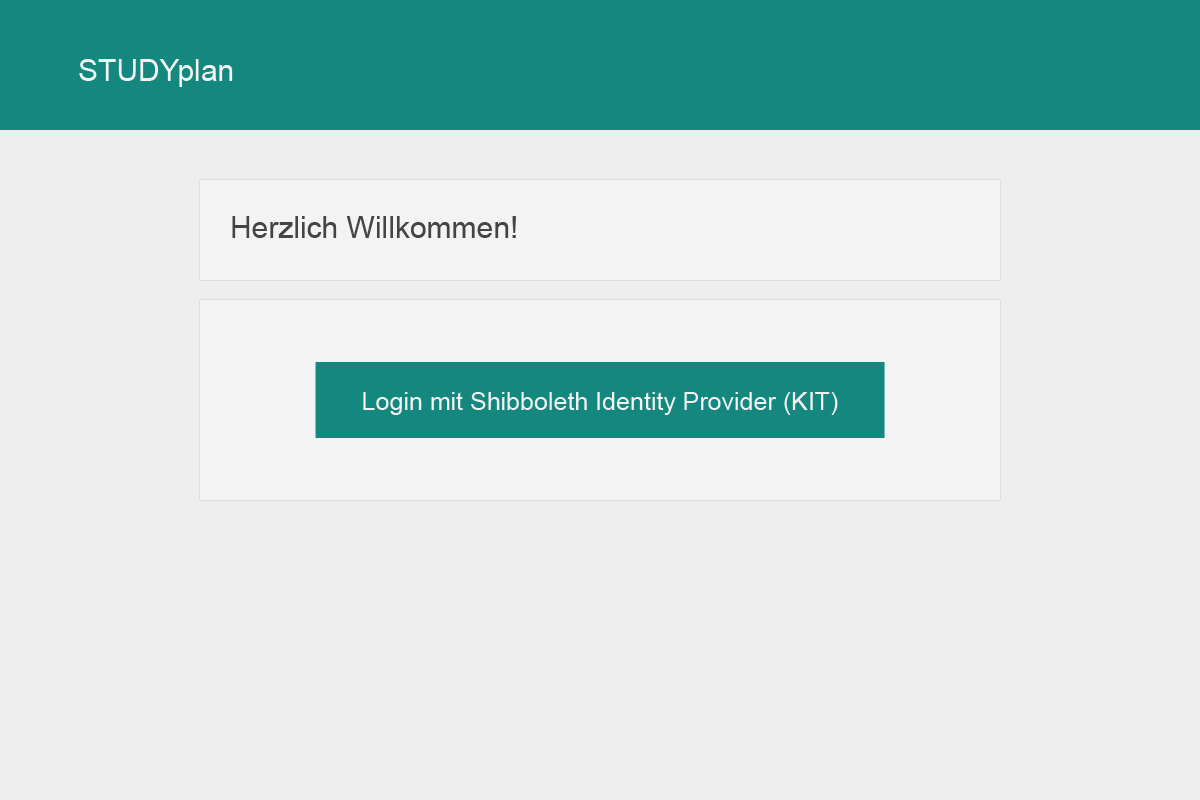
\includegraphics[width=0.7\textwidth]{../GUI/ergebnisse/login-1.png}
\end{figure}
Abbildung \ref{fig:gui-login-1} zeigt die Login-Seite. Diese sollte recht minimalistisch sein und lediglich die Möglichkeit bieten sich mit Hilfe des Shibboleth-Identity-Providers des KITs einloggen zu können.
\subparagraph{}
Loggt sich der Nutzer zum ersten Mal in das System ein wird er zum Registrierungs-Wizard (siehe Kapitel \ref{subsec:gui-registrierung}) weitergeleitet. Wenn er sich bereits zuvor schon einmal eingeloggt hat wird er auf die Hauptseite (siehe Kapitel \ref{subsec:gui-hauptseite}) weitergeleitet.
\subsection{Registrierungs-Wizard}
\label{subsec:gui-registrierung}
Nach dem Login wird man zum Registrierungs-Wizard weitergeleitet. Auf der ersten Seite (Abbildung \ref{fig:gui-registrierung-1}) wird der Nutzer dort nach grundlegenden Informationen wie dem Studiengang und dem Semester des Studienbeginns gefragt. Die Eingabe dieser Daten ist verpflichtend.
\subparagraph{}
Nachdem der Nutzer dann auf den Pfeil in der unteren Ecke geklickt hat, wird er auf die zweite Seite des Wizards (Abbildung \ref{fig:gui-registrierung-2}) weitergeleitet. Hier kann er angeben, welche Module er bereits begonnen und/oder abgeschlossen hat. 
Nach dem Bearbeiten der zweiten Seite des Wizards und dem Klick auf den Pfeil, wird der Nutzer auf die Hauptseite des Systems (siehe Kapitel \ref{subsec:gui-hauptseite}) weitergeleitet.
\subparagraph{}
Durch den Wizard soll sichergestellt werden, dass der Nutzer alle für das System relevanten Daten eingibt bevor er mit der Nutzung beginnt.
\begin{figure}[!htb]
	\caption{Erste Seite des Registrierungs-Wizard mit Eingabe von Studienfach und Studienbeginn}
	\label{fig:gui-registrierung-1}
	\centering
	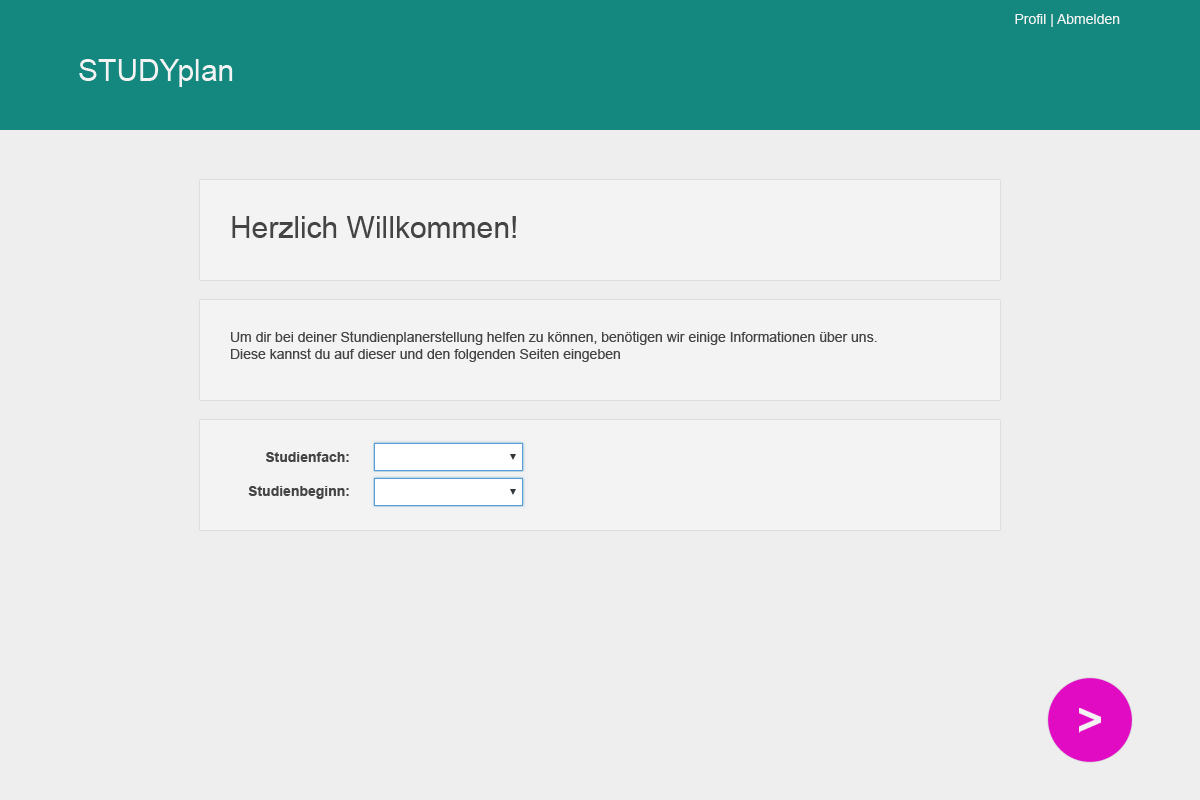
\includegraphics[width=0.7\textwidth]{../GUI/ergebnisse/registrierung-1.png}
\end{figure}

\begin{figure}[!htb]
	\caption{Zweite Seite des Registrierungs-Wizard mit Eingabe der schon begonnenen Module}
	\label{fig:gui-registrierung-2}
	\centering
	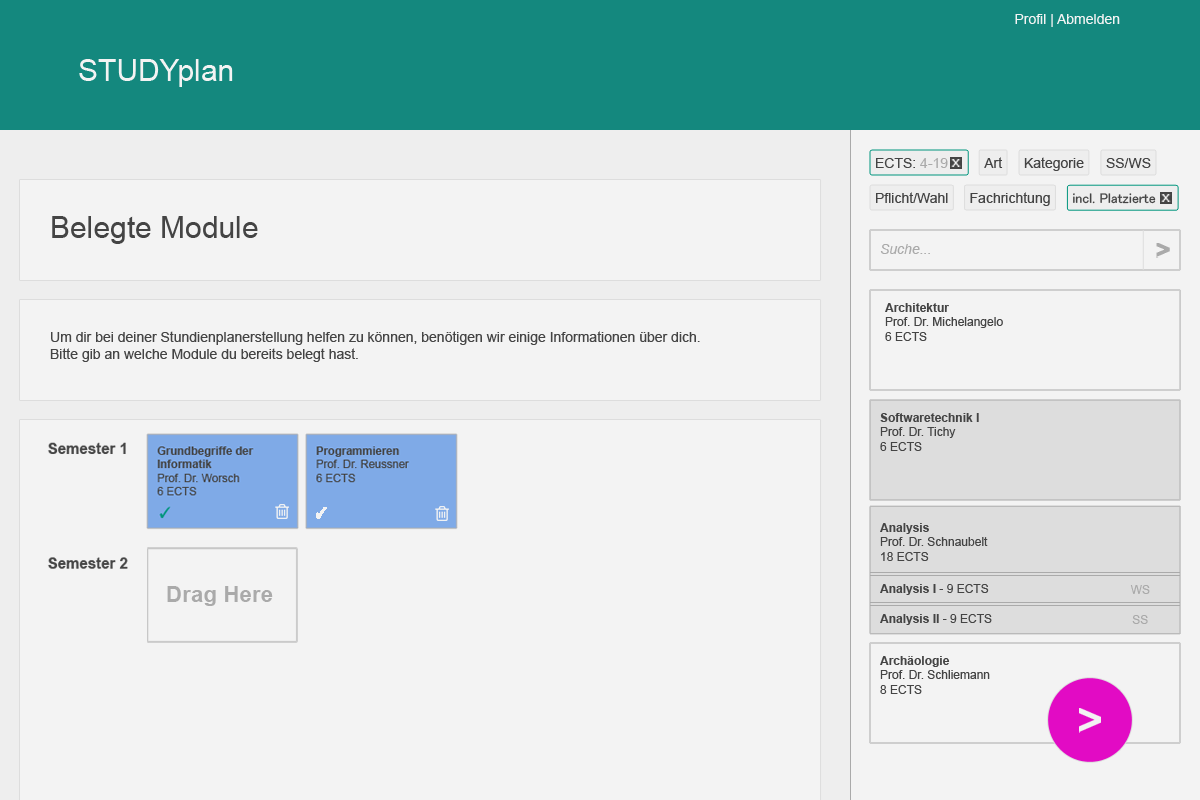
\includegraphics[width=0.7\textwidth]{../GUI/ergebnisse/registrierung-2.png}
\end{figure}


\subsection{Hauptseite}
\label{subsec:gui-hauptseite}
Die Hauptseite des Systems (Abbildung \ref{fig:gui-hauptseite-1}) stellt für den Nutzer die zentrale Anlaufstelle für alle Anwendungsfälle dar. Der Nutzer kann auf dieser Seite seine vorhandenen Studienpläne anzeigen, duplizieren, löschen sowie exportieren. Über das selektieren von mehreren Plänen, kann er auch Pläne vergleichen oder mehrere gleichzeitig löschen. Mittels des Plus-Buttons kann er darüber hinaus neue Pläne erstellen.\newline
Beim Klick auf "Anzeigen" wird der Nutzer auf die Seite zur manuellen Bearbeitung von Studienplänen (siehe Kapitel \ref{subsec:gui-manuelle-bearbeitung}) geleitet. Beim Klick auf das "+" wird er nach einem Namen für die Seite gefragt und anschließend ebenfalls auf die Seite zur manuellen Bearbeitung weitergeleitet.
\begin{figure}[!htb]
	\caption{}
	\label{fig:gui-hauptseite-1}
	\centering
	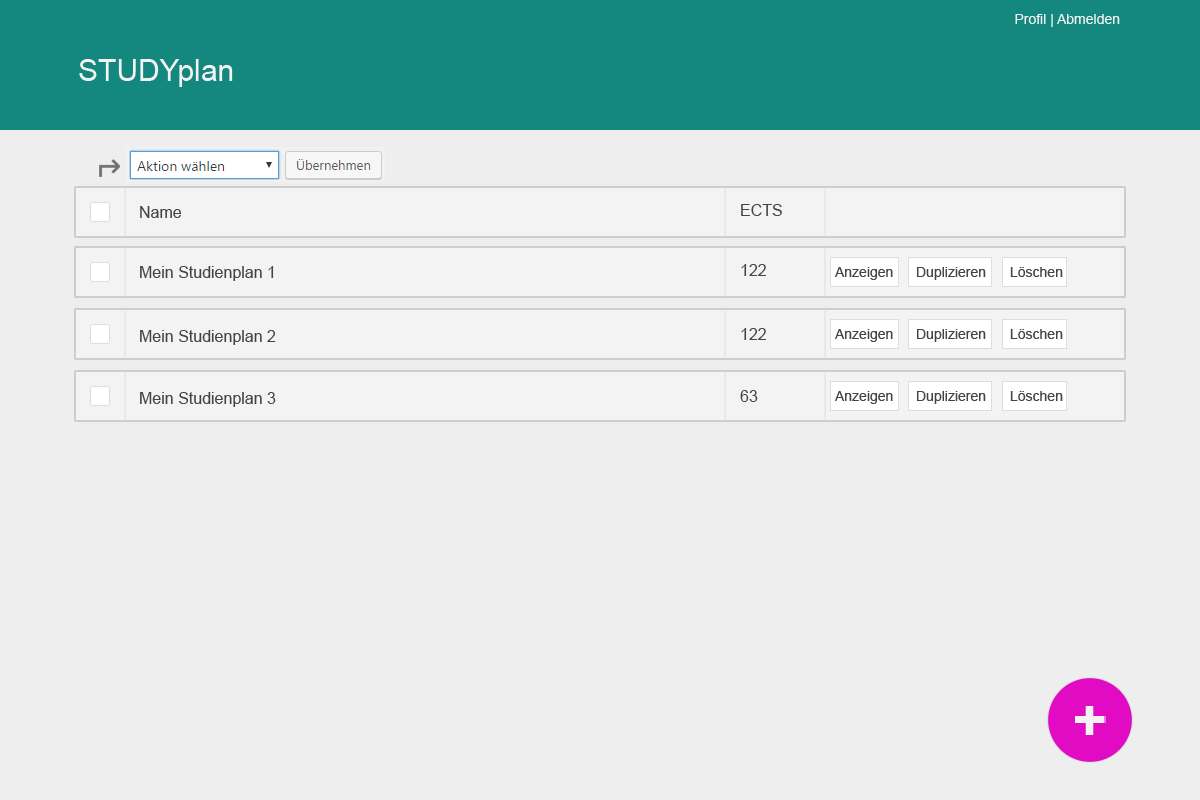
\includegraphics[width=0.7\textwidth]{../GUI/ergebnisse/hauptseite-1.png}
\end{figure}

\subsection{Manuelle Studienplan-Bearbeitung}
\label{subsec:gui-manuelle-bearbeitung}
In dieser Ansicht (Abbildung \ref{fig:gui-bearbeitung-1}) ist es dem Nutzer möglich, seinen Studienplan manuell zu bearbeiten. Hierfür kann er mittels Drag-and-Drop Module oder Teilmodule (z.B. das Teilmodul Analysis I in der Abbildung) in das gewünschte Semester zu ziehen. Hierdurch wird es dem Studienplan hinzugefügt.
\begin{figure}[!htb]
	\caption{}
	\label{fig:gui-bearbeitung-1}
	\centering
	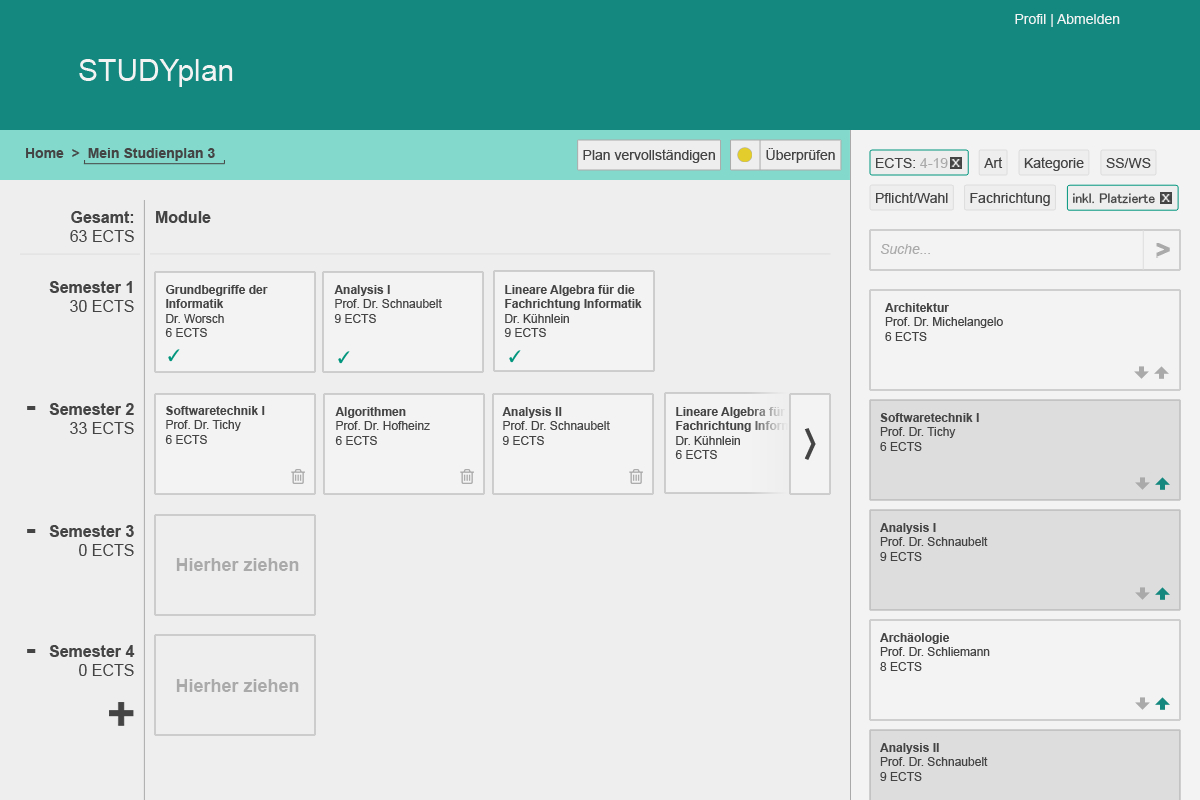
\includegraphics[width=0.7\textwidth]{../GUI/ergebnisse/bearbeitung-1.png}
\end{figure}

\subsubsection{Module filtern}
Module sind filterbar.
\begin{figure}[!htb]
	\caption{}
	\label{fig:gui-module-filtern-1}
	\centering
	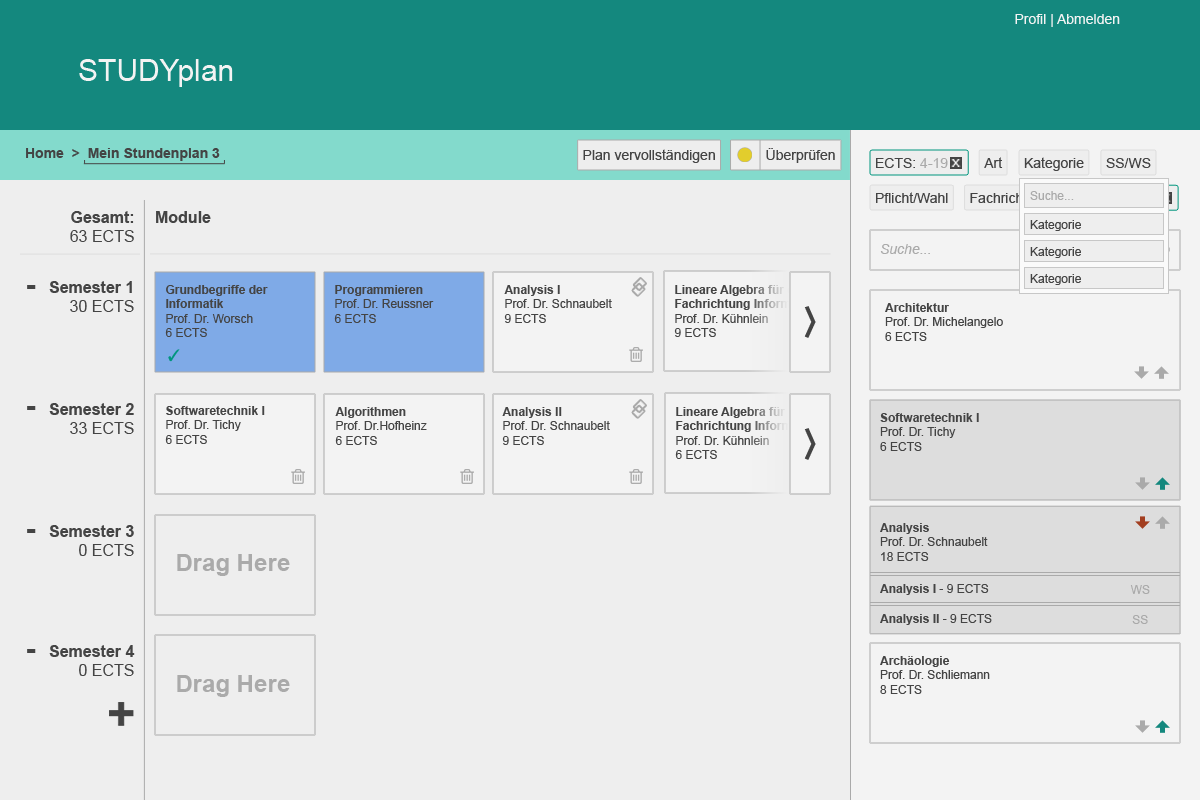
\includegraphics[width=0.7\textwidth]{../GUI/ergebnisse/module-filtern-1.png}
\end{figure}
\begin{figure}[!htb]
	\caption{}
	\label{fig:gui-module-filtern-2}
	\centering
	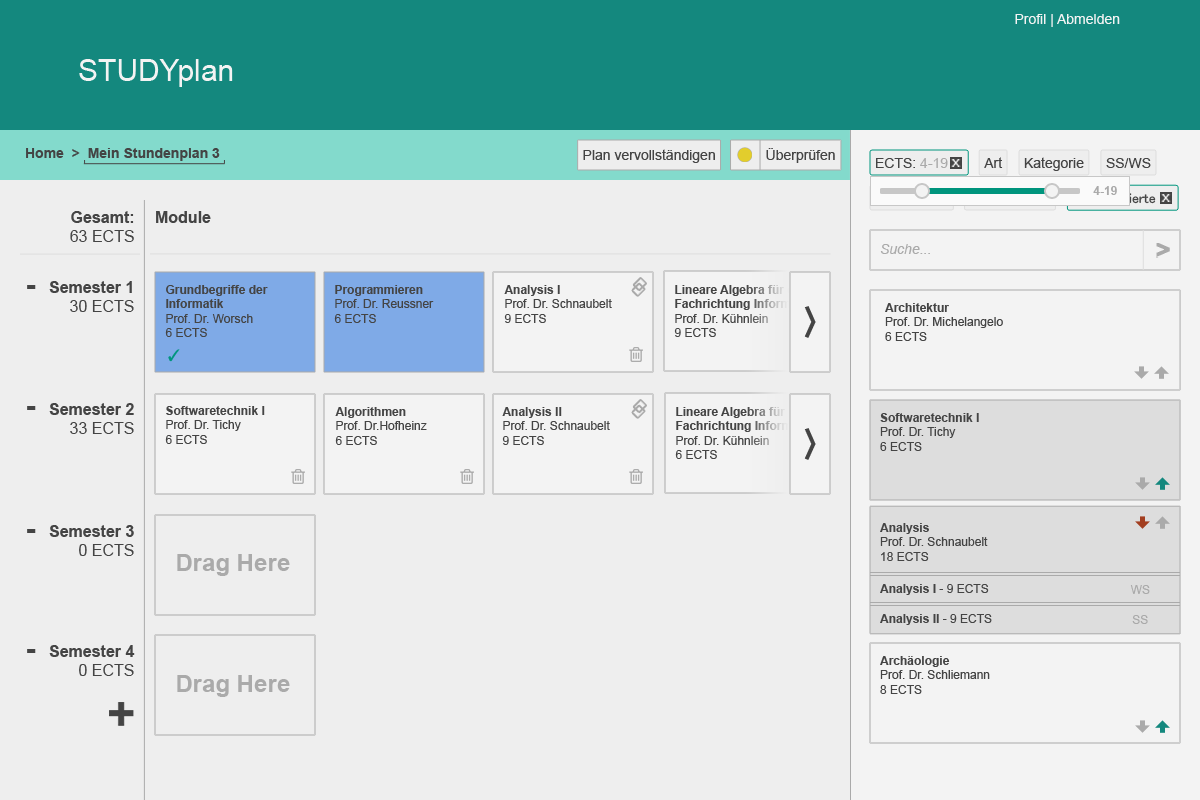
\includegraphics[width=0.7\textwidth]{../GUI/ergebnisse/module-filtern-2.png}
\end{figure}

\subsubsection{Modul-Informationen anzeigen}
Modulinformationen lassen sich auch anzeigen
\begin{figure}[!htb]
	\caption{}
	\label{fig:gui-modul-info-1}
	\centering
	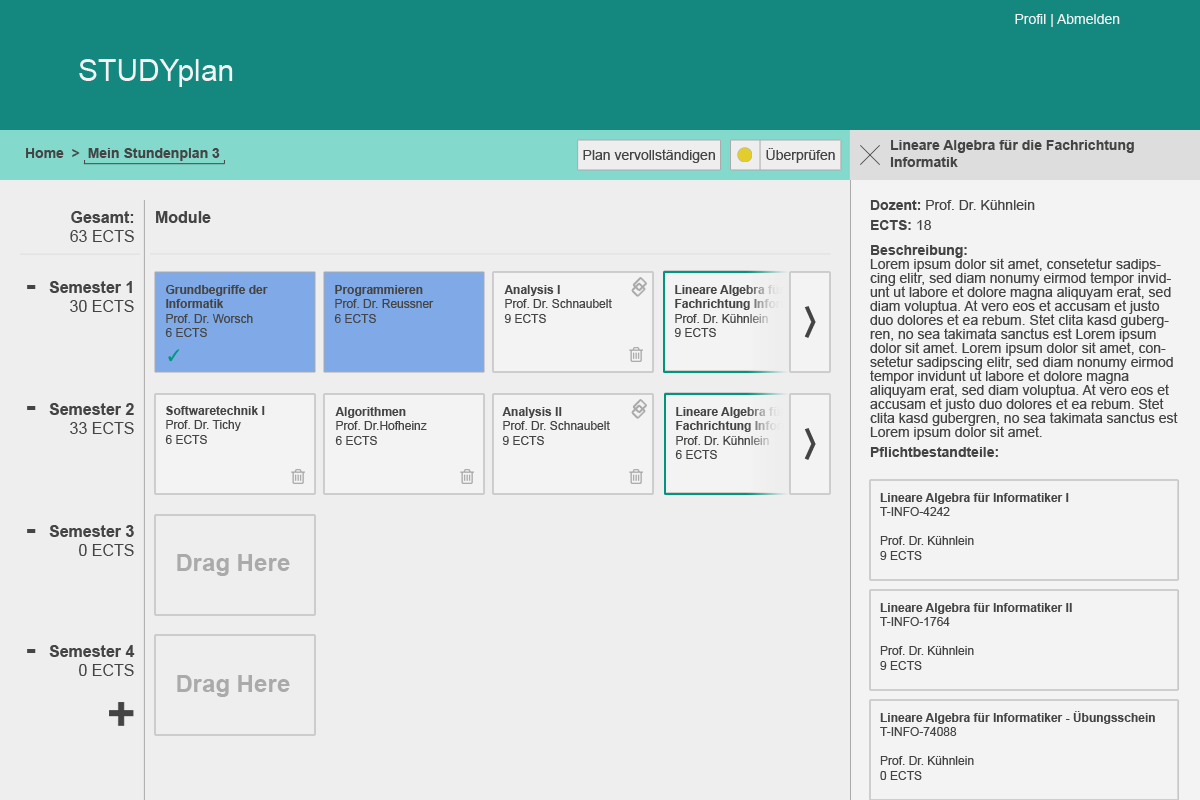
\includegraphics[width=0.7\textwidth]{../GUI/ergebnisse/modul-info-1.png}
\end{figure}


\subsection{Generierungs-Wizard}
Hier kann man Stundenpläne generieren.
\begin{figure}[!htb]
	\caption{}
	\label{fig:gui-generierung-1}
	\centering
	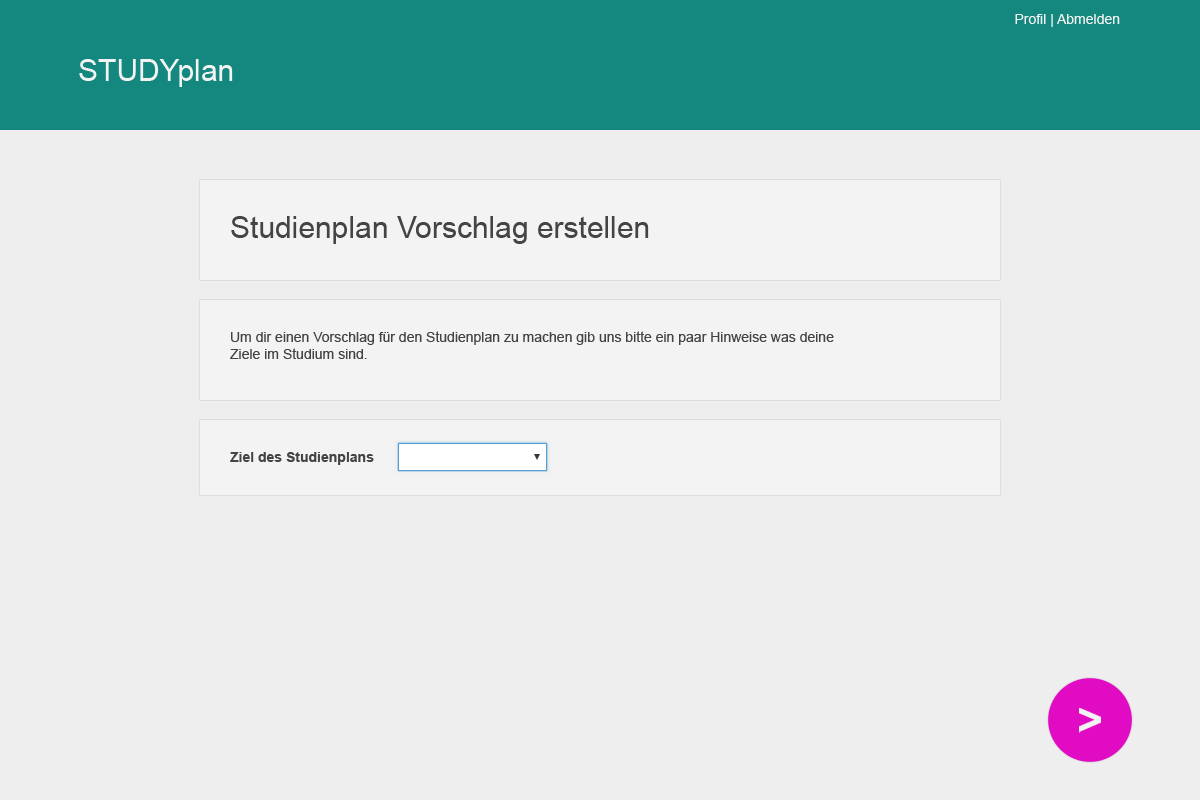
\includegraphics[width=0.7\textwidth]{../GUI/ergebnisse/generierung-1.png}
\end{figure}

\begin{figure}[!htb]
	\caption{}
	\label{fig:gui-generierung-2}
	\centering
	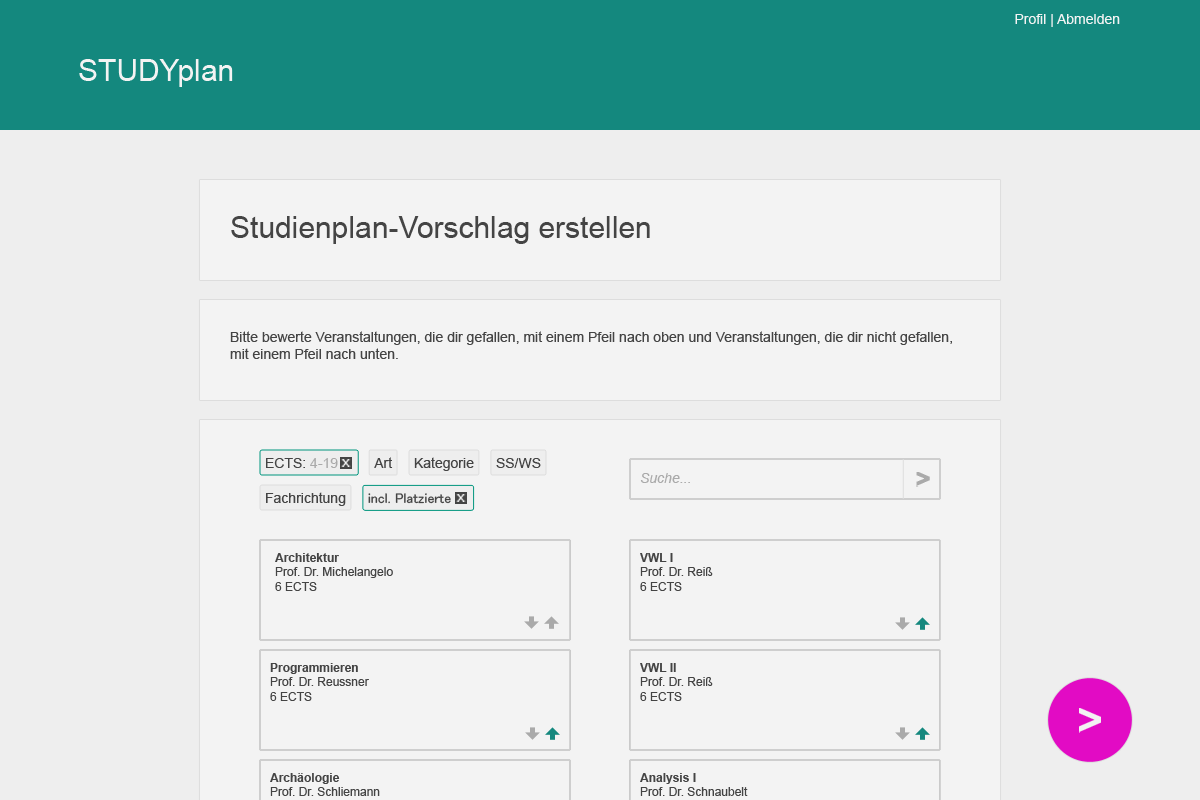
\includegraphics[width=0.7\textwidth]{../GUI/ergebnisse/generierung-2.png}
\end{figure}

\begin{figure}[!htb]
	\caption{}
	\label{fig:gui-generierung-3}
	\centering
	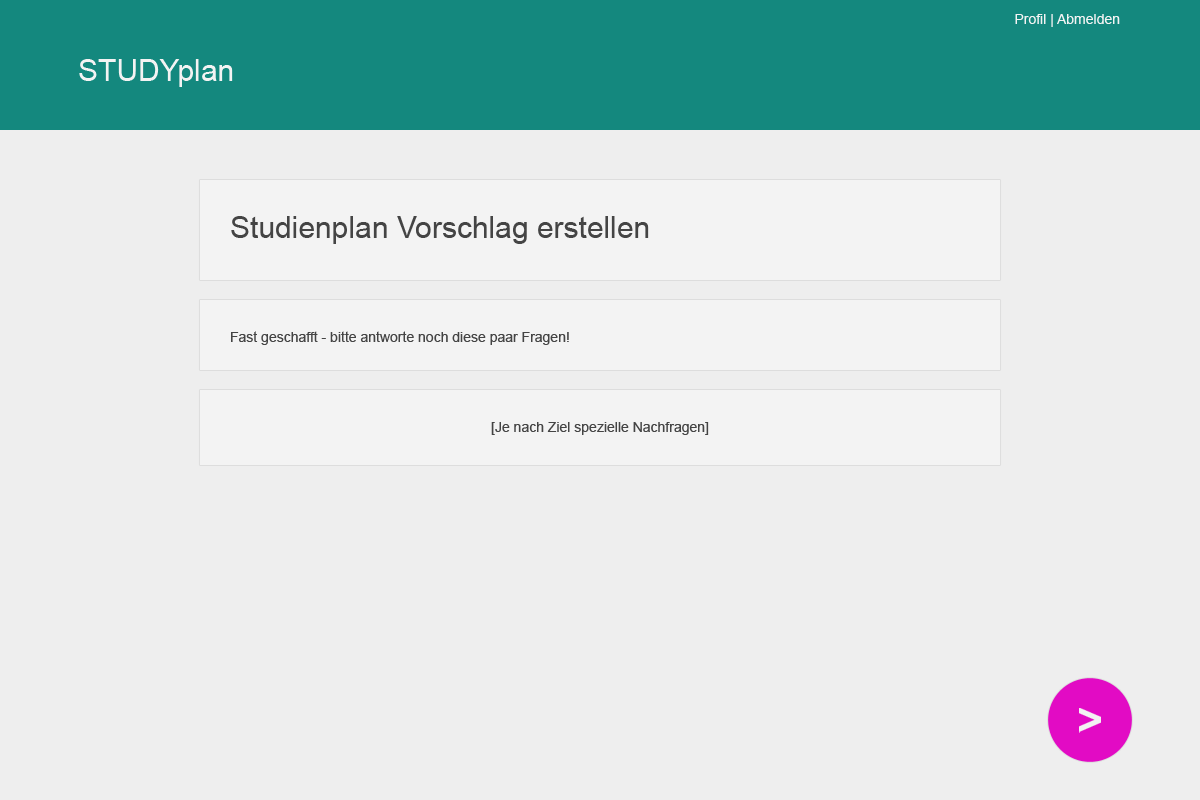
\includegraphics[width=0.7\textwidth]{../GUI/ergebnisse/generierung-3.png}
\end{figure}

\begin{figure}[!htb]
	\caption{}
	\label{fig:gui-generierung-4}
	\centering
	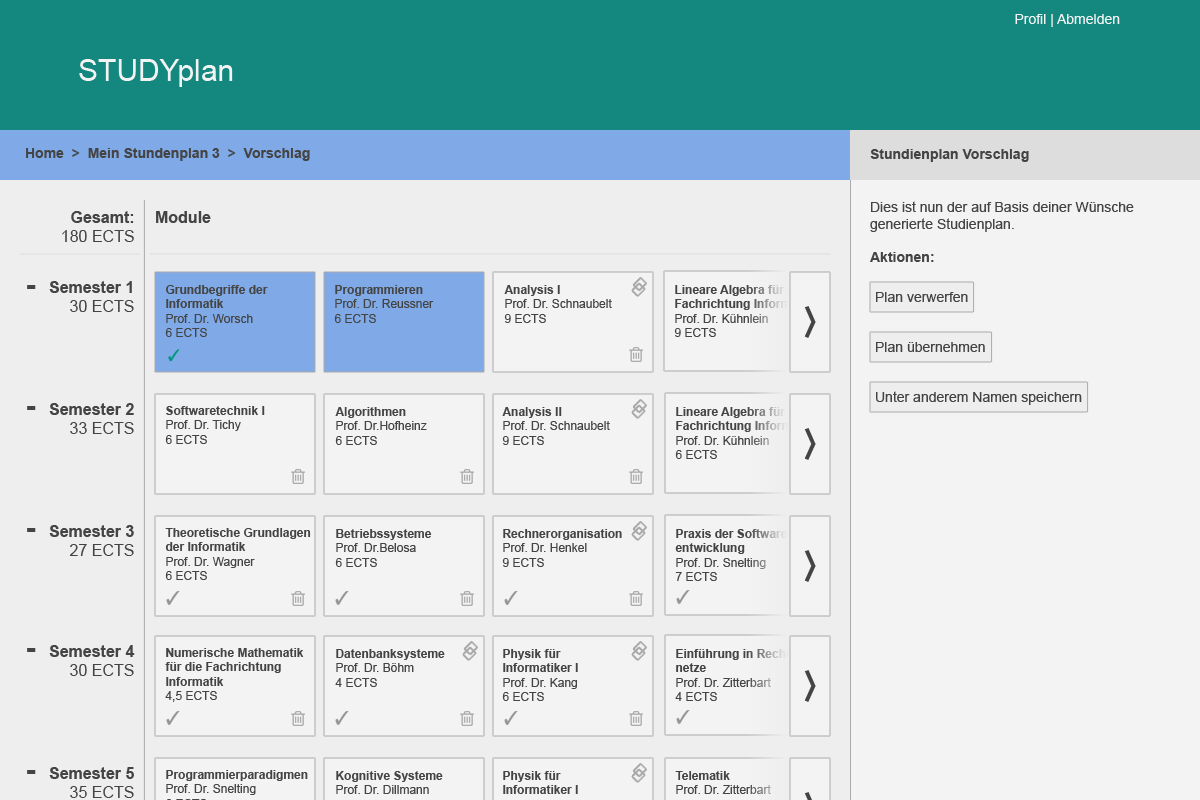
\includegraphics[width=0.7\textwidth]{../GUI/ergebnisse/generierung-4.png}
\end{figure}

\subsection{Verifizierung}
Verifizierung ist auch möglich mittels dieser Darstellung.
\begin{figure}[!htb]
	\caption{}
	\label{fig:gui-verifizierung-1}
	\centering
	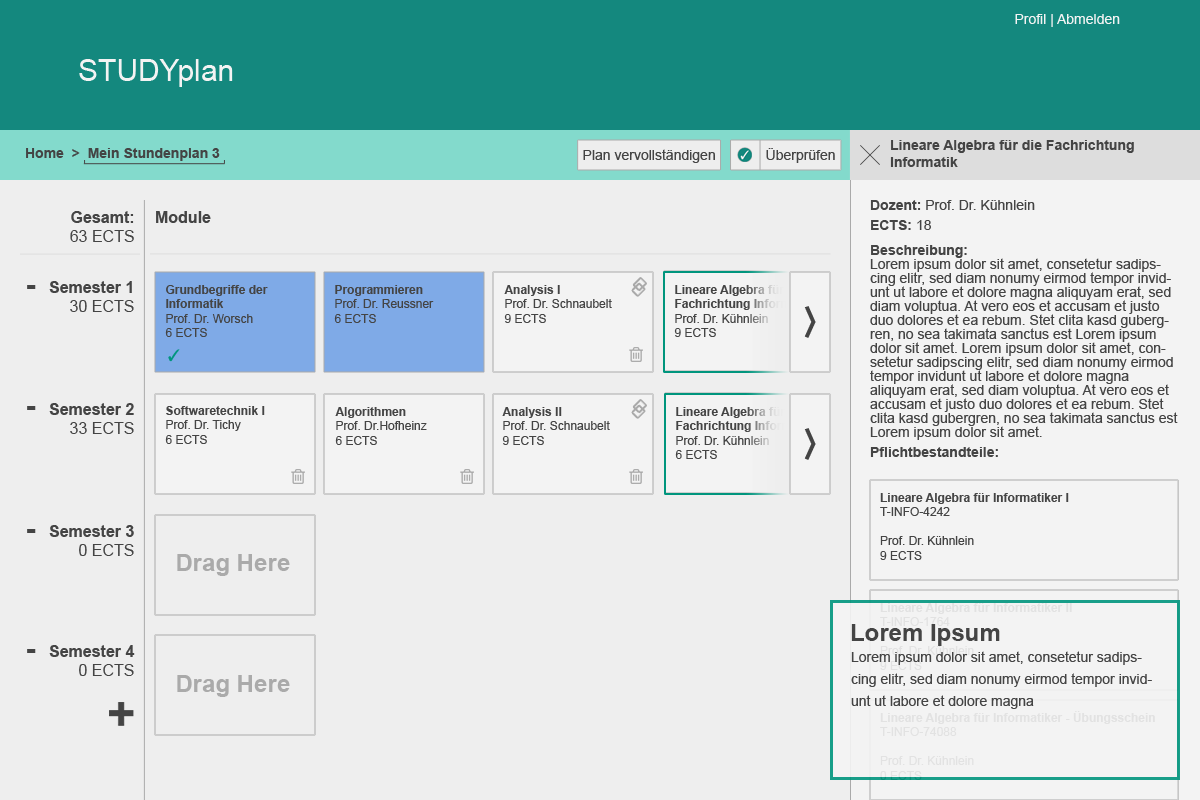
\includegraphics[width=0.7\textwidth]{../GUI/ergebnisse/verifizierung-1.png}
\end{figure}
\begin{figure}[!htb]
	\caption{}
	\label{fig:gui-verifizierung-2}
	\centering
	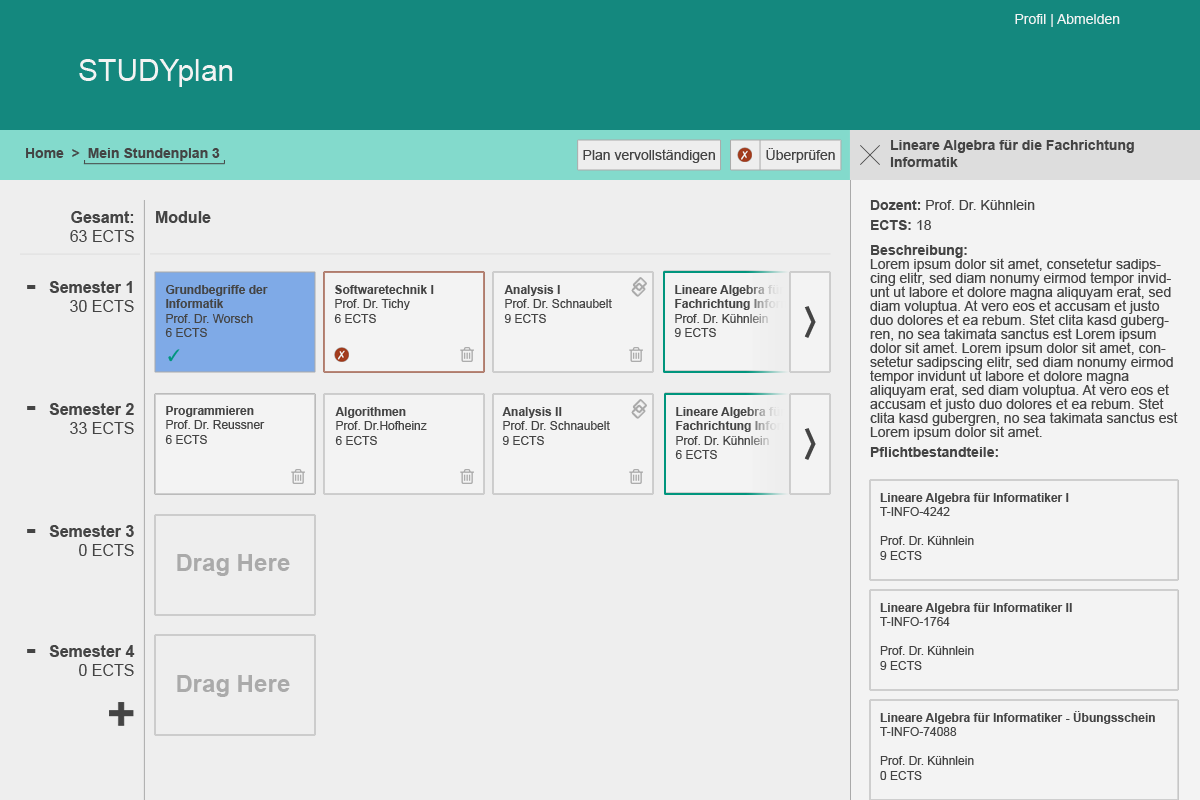
\includegraphics[width=0.7\textwidth]{../GUI/ergebnisse/verifizierung-2.png}
\end{figure}

\subsection{Profil}
So sieht das Profil aus.
\begin{figure}[!htb]
	\caption{}
	\label{fig:gui-profil-1}
	\centering
	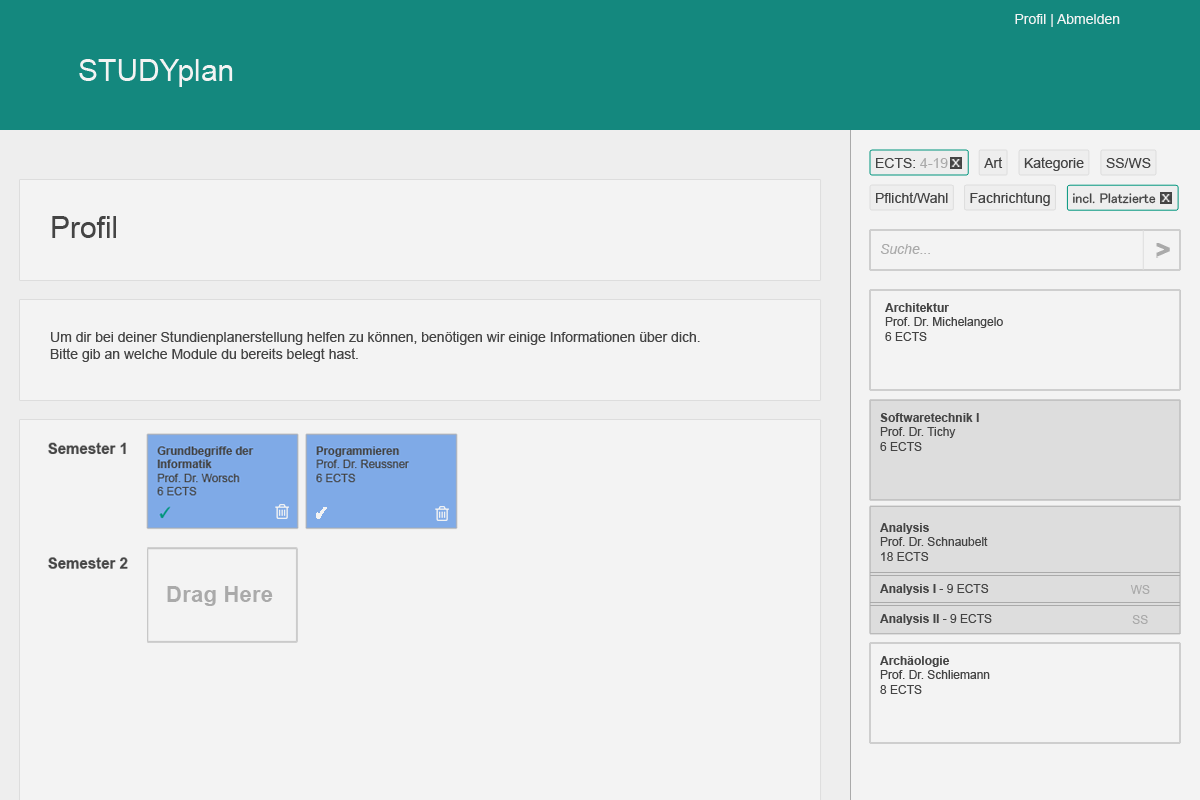
\includegraphics[width=0.7\textwidth]{../GUI/ergebnisse/profil-1.png}
\end{figure}

\section{Entwicklungs-Umgebung}

\subsection{Software}
	\subsubsection{Betriebssysteme}
	\subsubsection{Entwurf}
	\subsubsection{Implementierungstools}
	\subsubsection{Build-Tools}
	\subsubsection{Server-Software}
	\subsubsection{Entwurf}
	 	 
\subsection{Hardware}


%
% % Automatisch generiertes Glossar
%
%\glsaddall % das sorgt dafür, dass alles Glossareinträge gedruckt werden, nicht nur die verwendeten. Das sollte nicht nötig sein!
%
% % Glossareinträge
%
\newglossaryentry{Rest}
{
	name=REST,
	description={Abk. für Representational State Transfer, Programmierparadigma für \glspl{Webservice} auf Basis des HTTP-Protokolls}
}

\newglossaryentry{ECTS-Punkte}
{
	name=ECTS-Punkte,
	description={Leistungspunkte, die für ein erfolgreich absolviertes \gls{Modul} von der Hochschule auf Basis des ECTS-Punktesystems vergibt werden, und mit denen der Arbeitsaufwand gemessen wird},
}

\newglossaryentry{Generierungs-Tool}
{
	name=Generierungs-Tool,
	description={Tool, für die automatische Erstellung bzw. Vervollständigung von Studienpläne},
}


\newglossaryentry{Webservice}
{
	name=Webservice,
	plural=Webservices,
	description={Softwareanwendung, die über ein Netzwerk bereitgestellt wird}
}

\newglossaryentry{Plug-In-Paket}
{
	name=Plug-In-Paket,
	plural=Plug-In-Pakete,
	description={Paket bestehend aus mehreren \glspl{Plug-In}}
}

\newglossaryentry{iMage}
{
	name={iMage},
	description={Bildbearbeitungssoftware der Firma SWT. Bietet im Basispaket nur Funktionalitäten zur Skalierung und Drehung von Bildern}
}

\newglossaryentry{Internetbrowser}
{
	name={Internetbrowser},
	description={Programm, mit dem Websites gefunden, gelesen und verwaltet werden können, mit aktiviertem JavaScript}
}

\newglossaryentry{Online-Shop}
{
	name={Online-Shop},
	description={Internetseite, die Produkte zum Kauf anbietet}
}

\newglossaryentry{KIT}
{
	name=KIT,
	description={Das Karlsruher Institut für Technologie ist die Forschungsuniversität in der Helmholtz-Gemeinschaft. Standort der Universität ist Karlsruhe. }
}

\newglossaryentry{SCC}
{
	name=SCC,
	plural=SCC,
	description={Das Steinbuch Center for Computing ist ein Institut und das zentrale Rechenzentrum des \gls{KIT}s.}
}

\newglossaryentry{Benutzer}
{
	name=Benutzer,
	plural=Benutzer,
	description={Ein am \gls{KIT} eingeschriebener Student, der über ein gültigen Account beim \gls{SCC} verfügt.}
}

\newglossaryentry{Wizard}
{
	name=Wizard,
	plural=Wizards,
	description={Ein Wizard ist ein Subsystem, welches einen \gls{Benutzer} visuell durch eine Systemfunktionalität führt und dabei vom \gls{Benutzer} bestimmte Interaktionen mit dem System fordert.}
}

\newglossaryentry{Drag-and-Drop}
{
	name=Drag-and-Drop,
	description={(deutsch: "Ziehen und Ablegen") Eine Methode zur Bedienung grafischer Benutzeroberflächen bei der grafische Elemente mittels eines Mauszeigers bewegt werden.}
}

\newglossaryentry{Shibboleth Identity Provider}
{
	name=Shibboleth Identity Provider,
	description={Ein genau spezifiziertes System zum Login mittels einer von einer dritten Instanz bereitgestellten Identität.}
}

\newglossaryentry{Studiengang}
{
	name=Studiengang,
	description={Ein vom KIT angebotener, auf einer Studien- und Prüfungsordnung und einem Modulhandbuch basierender Studiengang.}
}

\newglossaryentry{Semester des Studienbeginns}
{
	name=Semester des Studienbeginns,
	description={Das Semester in welchem der \gls{Benutzer} im ersten Fachsemester des \gls{Studiengang}s war.}
}

\newglossaryentry{Modul}
{
	name=Modul,
	plural=Module,
	description={Ein Modul ist ein Teilblock des Studiums, welcher aus verschiedenartigen Veranstaltungen (genannt \glspl{Teilmodul}) bestehen kann und für welchen man nach Ablegung eventueller \glspl{Modulpruefung} eine festgelegte Anzahl an ECTS-Punkten erhält.}
}
\newglossaryentry{Teilmodul}
{
	name=Teilmodul,
	plural=Teilmodule,
	description={Ein Teilmodul ist eine universitäre Veranstaltung, welche als Teil eines Moduls besucht werden kann und mittels einer (wie auch immer gearteten) \gls{Modulpruefung} bestanden werden kann.}
}
\newglossaryentry{Modulpruefung}
{
	name=Modulprüfung,
	plural=Modulprüfungen,
	description={Eine Modulprüfung ist eine Prüfung, welche abgelegt werden muss um ein Modul \glslink{Modul abgeschlossen}{abzuschließen}.}
}
\newglossaryentry{Zur Pruefung angetreten}
{
	name=Zur Pruefung angetreten,
	description={Ein \gls{Benutzer} ist zu einer \gls{Modulpruefung} angetreten, wenn er sich fristgerecht für selbige angemeldet und nicht fristgerecht abgemeldet hat.}
}

\newglossaryentry{Modul abgeschlossen}
{
	name=Modul abgeschlossen,
	description={Ein \gls{Modul} gilt als abgeschlossen, wenn der \gls{Benutzer} alle nach Modulhandbuch notwendigen \glspl{Modulpruefung} bestanden hat.}
}

\newglossaryentry{Modul begonnen}
{
	name=Modul begonnen,
	description={Ein \gls{Modul} gilt als begonnen, wenn der \gls{Benutzer} zu mindestens einer \gls{Modulpruefung} \glslink{Zur Pruefung angetreten}{angetreten} ist.}
}

\newglossaryentry{Studienplan}
{
	name=Studienplan,
	plural=Studienpläne,
	description={Eine Zusammenstellung von Modulen, in welcher enthalten ist wann welches Modul planmäßig \glslink{Modul begonnen}{begonnen} werden soll.}
}

\end{document}
